\documentclass{article}
\usepackage{graphicx}
\usepackage[font=small, labelfont=bf, justification=centering]{caption}
\usepackage[colorlinks=true, linkcolor=black, urlcolor=red, citecolor=black]{hyperref}
\usepackage[a4paper, margin=1in]{geometry}
\usepackage{amsmath}
\usepackage{mathtools}

\begin{document}
  {\centering \textbf{Problem 1.} \par}
  A line passing through the incenter $I$ of the triangle $ABC$ intersect
  its incircle at $D$ and $E$ and its circumcircle at $F$ and $G$, in such
  a way that the point $D$ lies between $I$ and $F$. Prove that:
  $DF \cdot EG \geq r^{2}$.

  \medskip

  {\centering \textbf{Solution} \par}
  \begin{figure}[h]
    \centering
    \begin{minipage}{0.4\textwidth}
      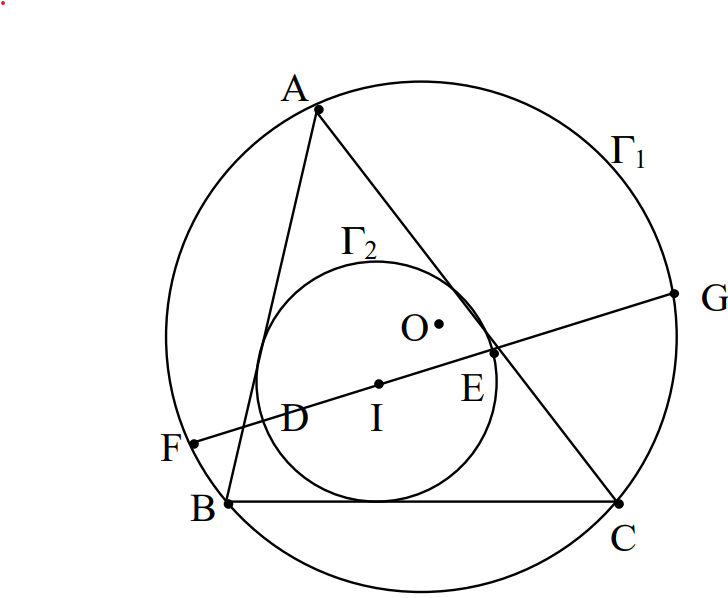
\includegraphics[width=\linewidth]{first.png}
      \caption{An illustration of the first problem. \href{https://www.obm.org.br/content/uploads/2017/01/eixos-2.pdf}{Source}}
    \end{minipage}
    \hfill
    \begin{minipage}{0.5\textwidth}
      \begin{align*}
        &DF \cdot EG = (IF - ID)(IG - IE) = (IF - r)(IG - r) \\
        &\text{where } r \text{ is the inradius. Hence} \\
        &IF \cdot IG - r(IF + IG) + r^2 = - Pot_{\Gamma_{1}} I - GFr + r^2 \\
        &= R^2 - IO^2 - GFr + r^2. \\
        &\text{Since the distance } IO \text{ between the incenter and} \\
        &\text{circumcenter satisfies } IO = \sqrt{R^2 - 2Rr}, \text{ it follows} \\
        &R^2 - IO^2 - GFr + r^2 = 2Rr - GFr + r^2 \Rightarrow 2Rr \\
        &- GFr + r^2 \geq r^2 \iff 2R r \geq GFr. \\
        &\text{This inequality holds since } GF \text{ is a chord of } \Gamma_1. \\
        &DF \cdot EG = r^2 \iff 2Rr = GFr.
      \end{align*}
    \end{minipage}
  \end{figure}

  \rule{\linewidth}{0.4pt}

  {\centering \textbf{Problem 2.} \par}

  \medskip

  {\centering \textbf{Solution} \par}
\end{document}
